\usetikzlibrary{snakes, patterns}
\tikzstyle{ground}=[fill,pattern=north east lines,draw=none,minimum width=1,minimum height=1]
\tikzstyle{spring}=[snake=coil,segment length=2mm, segment amplitude=2mm]

\part{力学}
为了简化问题,我们可以将物体抽象成质点,质点具有质量,在每个时刻都有一个的位置,没有形状和体积。还可以视为不能发生变形的刚体,不可压缩且没有内摩擦的理想流体,理想弹性体等等。为了方便讨论,我们一般只讨论质点。
多个物体在一起被称为系统,系统在一些情况下整体也可以被看成一个物体。

例如汽车在真实道路上行驶时,只需要计算路程、时间、速度时,可以将路线化为直线,而汽车为一个质点

\chapter{运动学}
\section{标量和矢量}
在物理学中,有些量只有大小没有方向,称为标量;有些量既有大小也有方向,称为矢量。量的值称为量值,标量的值可以用数和单位表示,矢量的值可以用向量和单位表示。数学上向量主要有两种表达形式,使用直角坐标下的各分量表示或使用模和方向表示。可以把向量的模和单位放在一起,方向单独表示。

以下是一些例子: \\
标量:$1kg$, $3m$ \\
矢量:$5N$,右向上$60^\circ$, $(5\bm{i}+2\bm{j})N$ \\

\section{位置、位移和路程}
为了表示位置,通常选取一个点作为参考,建立坐标系来进行描述。直线运动可以使用一维坐标系,平面曲线运动可以使用二维直角坐标系,极坐标系等。本书一般不涉及空间曲线运动。

\section{时间间隔和时刻}
时刻可以用于表示某个事件的发生时间,时间间隔可以用于表示两个事件的时间差。
时刻无法直接表示,通常选取一个事件作为参考时刻,与参考时刻的时间差来表达时刻。物理中通常使用“初始时刻”表示该参考时刻。按照传统习惯,日常生活中通常使用与天文现象一定程度上相关的历法表示日期,又把一天内的时间通过时、分、秒来描述。

\section{速度和速率}
速度(vecoly)是描述物体运动快慢的物理量,有方向和大小,
\begin{equation}\label{vdef}
\bm{v}=\frac{\Delta \bm{x}}{\Delta t}
\end{equation},速度的大小又称为速率(speed)。

匀速直线运动是指,速度不为零,且速度的大小和方向都不发生变化的运动

\section{加速度}
加速度是速度随时间的变化率,速度变化的越快,加速度的大小越大
\begin{equation}\label{adef}
\bm{a}=\frac{\Delta \bm{v}}{\Delta t}
\end{equation}

匀变速直线运动是指,加速度不为零,且加速度的大小和方向都不发生变化的运动。
匀变速直线运动又可以分为匀加速直线运动和匀减速直线运动。

由于匀变速直线运动的速度不断变化,因此不能将$v=at$代入$s=vt$来计算路程,

\begin{wrapfigure}{l}{0cm}
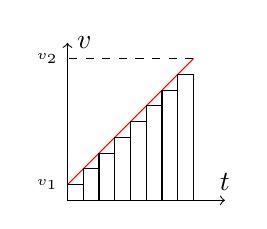
\begin{tikzpicture}[scale=0.2,domain=0:8]
	\draw[->](0,0)--(10,0)node[left,above]{$t$};
	\draw[->](0,0)--(0,10)node[right]{$v$};
	\draw[color=red] plot(\x,1+\x);
	\draw (0,0) rectangle(1,1);
	\draw (1,0) rectangle(2,2);
	\draw (2,0) rectangle(3,3);
	\draw (3,0) rectangle(4,4);
	\draw (4,0) rectangle(5,5);
	\draw (5,0) rectangle(6,6);
	\draw (6,0) rectangle(7,7);
	\draw (7,0) rectangle(8,8);
	\draw (0,1) node[left, font=\tiny]{$v_1$};
	\draw[dashed] (8,9)--(0,9) node[left, font=\tiny]{$v_2$};
\end{tikzpicture}
\end{wrapfigure}

在$v-t$图像中,可以通过分段近似求每段的路程,每段路程的长度就对应于矩形面积,当每段持续时间越来越小时,面积之和就越来越接近矩形面积,当持续时间趋向0时,路程就对应于梯形面积。因此$s=\frac{v_1+v_2}{2}t$,根据式(\ref{adef})此时的加速度为$a=\frac{v_2-v_1}{t}$,综合两式可得
\begin{equation}\label{consta_path}
s=\frac{v_2^2-v_1^2}{2a}
\end{equation}

汽车刹车时,如果加速度一直为$a$,初速度$v_0$,刹车后静止,制动距离应为$s=\frac{v_0^2}{2a}$。相同加速度下,两倍速度下的刹车距离就变为原来的四倍了。

\chapter{静力学}
\section{常见的力}
按照力的性质可分:重力,摩擦力,弹力
力的作用位置可分:外力和内力
外力按照是否接触可分:接触力(如摩擦力)和非接触力(如磁力)
外力按照作用位置又可分:表面力(仅仅是表面)和体积力(作用于物体内部)

\section{力的运算法则}
\begin{wrapfigure}{l}{0cm}
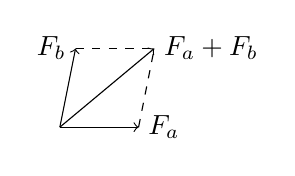
\begin{tikzpicture}[scale=1]
	\draw[->](0,0)--(1,0)node[right]{$F_a$};
	\draw[->](0,0)--(0.2,1)node[left]{$F_b$};
	\draw[->](0,0)--(1.2,1)node[right]{$F_a+F_b$};
	\draw[dashed](1,0)--(1.2,1);
	\draw[dashed](0.2,1)--(1.2,1);
\end{tikzpicture}
\end{wrapfigure}
作用于同一点的力相加符合平行四边行法则


练习:\\
1. 画出以下力的合力并计算大小
\begin{tabbing}
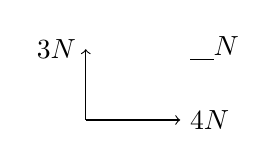
\begin{tikzpicture}[scale=0.3]
	\draw[->](0,0)--(4,0)node[right]{$4N$};
	\draw[->](0,0)--(0,3)node[left]{$3N$};
	\draw (4,3)node[right]{$\underline{\hbox to 3mm{}}N$};
\end{tikzpicture}
\end{tabbing}


\section{平衡}
平衡是指质点虽受外力,但仍然保持静止或匀速直线运动状态。如果只有一组力的作用下,物体仍然保持平衡,这组力被称为一组平衡力。

\begin{wrapfigure}{l}{0cm}
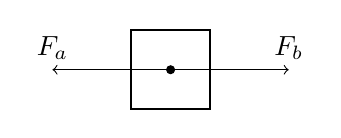
\begin{tikzpicture}[scale=1]
	\draw[thick](0,0)rectangle(1,1);
	\draw[fill](0.5, 0.5)circle[radius=0.5mm];
	\draw[->](0.5,0.5)--(-1,0.5)node[above]{$F_a$};
	\draw[->](0.5,0.5)--(2,0.5)node[above]{$F_b$};
\end{tikzpicture}
\end{wrapfigure}
二力平衡原理
作用在同一质点上的两个大小相等,方向相反的力平衡。这两个力被称为一对平衡力。

练习:\\
1. 判断以下力是否是平衡力\\
\begin{tabbing}
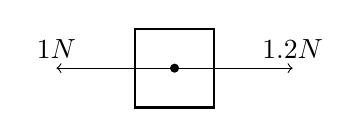
\begin{tikzpicture}[scale=1]
	\draw[thick](0,0)rectangle(1,1);
	\draw[fill](0.5, 0.5)circle[radius=0.5mm];
	\draw[->](0.5,0.5)--(-1,0.5)node[above]{$1N$};
	\draw[->](0.5,0.5)--(2,0.5)node[above]{$1.2N$};
\end{tikzpicture}

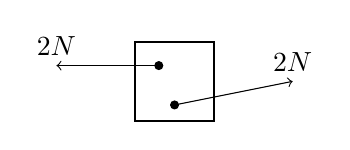
\begin{tikzpicture}[scale=1]
	\draw[thick](0,0)rectangle(1,1);
	\draw[fill](0.3, 0.7)circle[radius=0.5mm];
	\draw[fill](0.5, 0.2)circle[radius=0.5mm];
	\draw[->](0.3,0.7)--(-1,0.7)node[above]{$2N$};
	\draw[->](0.5,0.2)--(2,0.5)node[above]{$2N$};
\end{tikzpicture}

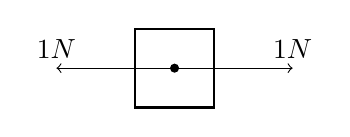
\begin{tikzpicture}[scale=1]
	\draw[thick](0,0)rectangle(1,1);
	\draw[fill](0.5, 0.5)circle[radius=0.5mm];
	\draw[->](0.5,0.5)--(-1,0.5)node[above]{$1N$};
	\draw[->](0.5,0.5)--(2,0.5)node[above]{$1N$};
\end{tikzpicture}
\end{tabbing}

\section{虎克定律}
\begin{wrapfigure}{l}{0cm}
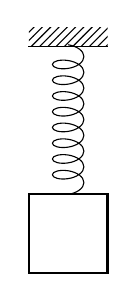
\begin{tikzpicture}
	\node (wall1) [ground, minimum width=1cm] {};
    \draw (wall1.south west) -- (wall1.south east);
	\draw[spring](0,-0.1)--(0,-2);
	\draw[thick] (-0.5,-2) rectangle (0.5,-3);
\end{tikzpicture}
\end{wrapfigure}
处于平衡状态时,弹簧下端受到的拉力大小等于物体的重力。测量弹簧的长度,更换不同质量的物体,进行多次测量。可发现物体质量与弹簧伸长量正比。

在弹性限度内,弹簧偏离平衡位置的距离与作用在弹簧上的力与成正比。

观察弹簧测力计的刻度,能发现刻度是均匀的,这是一种虎克定律的应用。

\begin{equation}
\bm{F}=k\bm{x}
\end{equation}

练习:\\
1. 某弹簧水平静止状态长度$5cm$,在弹性限度内,施加$1N$的拉力后长度为$6cm$,现在弹簧长度为$4.5cm$,请问施加的压力应为$\underline{\hbox to 7mm{}}$


\chapter{动力学}
\section{自由落体运动}
\begin{definition}
自由落体是指初速度为0的运动,只受重力的运动
\end{definition}

亚里斯多德曾经提出物体越重,下落速度快。伽利略提出,如果有两种轻重不同的石头分别下落和捆绑一起后下落,捆绑后整体可以视为一个更重的物体,按照亚里斯多德的观点,应该是$v_{\text{轻}}<v_{\text{重}}<v_{\text{合}}$。但是这不符合日常经验,应该是较快物体被较慢物体拖累,最终形成的共同速度应该介于较快物体和较慢物体的速度之间,即$v_{\text{轻}}<v_{\text{合}}<v_{\text{重}}$,产生了矛盾。

\begin{tabbing}

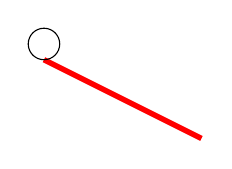
\begin{tikzpicture}[scale=1]
	\draw[line width=2pt, color=red] (0,1)--(2,0);
	\draw (0, 1.2) circle[radius=0.2];
\end{tikzpicture}

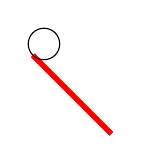
\begin{tikzpicture}[scale=1]
	\draw[line width=2pt, color=red] (0,1)--(1,0);
	\draw (0.2/1.4, 1+0.2/1.4) circle[radius=0.2];
\end{tikzpicture}

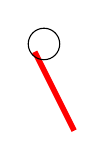
\begin{tikzpicture}[scale=1]
	\draw[line width=2pt, color=red] (0,1)--(0.5,0);
	\draw (0.2/1.7, 1.1) circle[radius=0.2];
\end{tikzpicture}

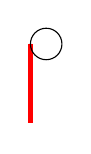
\begin{tikzpicture}[scale=1]
	\draw[line width=2pt, color=red] (0,1)--(0,0);
	\draw (0.2, 1.0) circle[radius=0.2];
\end{tikzpicture}

\end{tabbing}
在历史上,伽利略进行斜面实验,外推出自由落体的规律。当时的科技水平无法精确观察自由落体运动,只能采用这种方式


\section{牛顿运动定律}
\subsection{牛顿第一定律}
一切物体将保持静止或匀速直线运动状态,除非有外力使它改变运动状态

\subsection{牛顿第二定律}
\begin{equation}\label{newtown2}
\bm{F}=m\bm{a}
\end{equation}
通过实验可以验证,$m$是物体质量,其中$\bm{F}$是物体的合外力 \\
\paragraph{例1}
用弹簧测力计拉着一个物体进行变速运动,观察弹簧测力示速与物体运动之间的关系

\subsection{牛顿第三定律}
